\label{appendix-c}
Figure~\ref{fig:traceability_map} provides an end-to-end traceability view of the dissertation, linking the research problem to research questions, objectives, methods, results, implications, and the resulting contributions. The map is organized in columns that correspond to major components of the dissertation narrative. Nodes represent labeled elements such as research questions, objectives, and section-level methods and results topics, and directed links indicate traceability relationships between elements. Link weight visually distinguishes primary traceability relationships from supporting relationships. The intent of the map is to serve as a navigation and audit aid. Readers can start from any element of interest, follow links forward to identify the empirical evidence and derived implications that support it, or trace backward from a contribution to the specific results and methods that produced its supporting evidence.


% % \begin{landscape}
% \begin{figure}[p]
%   \centering
%   \resizebox{1.25\textwidth}{!}{
%   \begin{dot2tex}[neato,options=-tmath]
%     \input{research_traceability.dot}
%     \end{dot2tex}
%   }
%   \caption{Traceability map linking the research problem to research questions, objectives, methods, results, implications, and contributions.}
%   \label{fig:traceability_map}
% \end{figure}
% % \end{landscape}


\begin{figure}[p]
  \centering
\includegraphics[width=1.00\linewidth]{traceability-fig/research_traceability_v4.png}
  \caption{Traceability Map linking the research problem to research questions, objectives, methods, results, implications, and contributions}
  \label{fig:traceability_map}
\end{figure}


% \begin{figure}
%     \centering
%     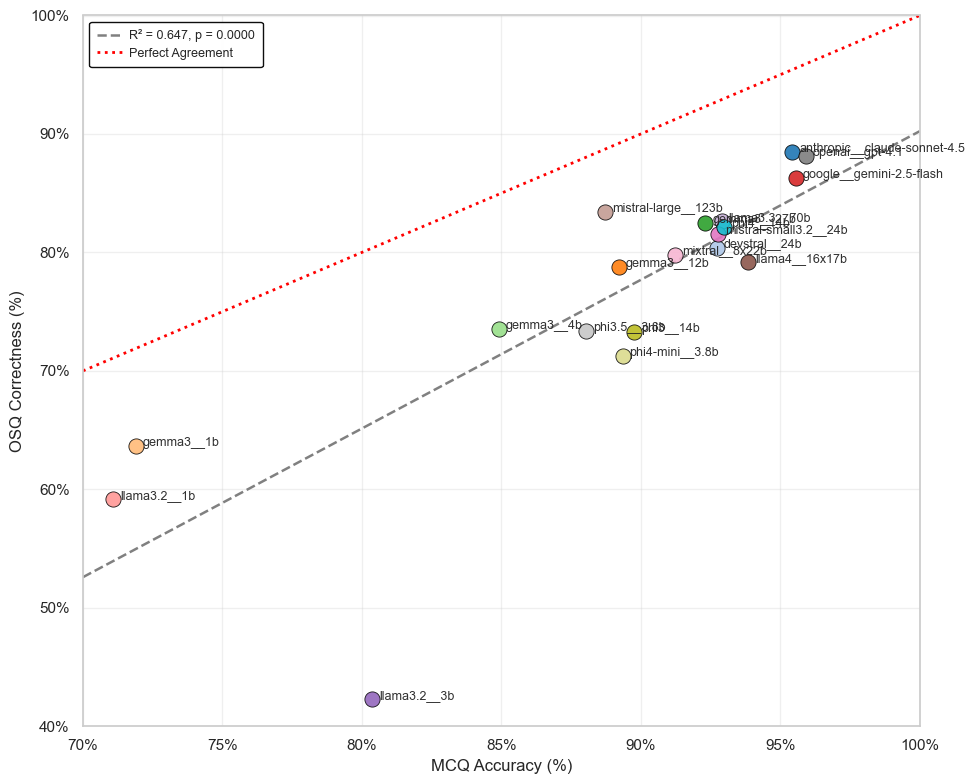
\includegraphics[width=0.90\linewidth]{figs/ch4/mcq_vs_osq_40-100_70-100.png}
%     \caption{MCQ Accuracy vs OSQ Mean Score: Global View}
%     \label{fig:mcq-vs-osq-global}
% \end{figure}

% \newpage
\clearpage























